%Styles
\tikzstyle{block} = [draw, thick, rectangle, minimum height=3em, minimum width=3em]
\tikzstyle{math} = [draw, thick, circle, minimum size=0.6cm,node distance=2cm, path picture={ 
      \draw[line] (path picture bounding box.south west) -- (path picture bounding box.north east);
      \draw[line] (path picture bounding box.north west) -- (path picture bounding box.south east);}]
\tikzstyle{gain} = [draw, thick, isosceles triangle, minimum size=0.6cm,node distance=1.5cm]
\tikzstyle{pt} = [coordinate]
\tikzstyle{line} = [->,thick]
\tikzstyle{ground}=[color=gray,postaction={draw,decorate,decoration={border,angle=-45,amplitude=0.2cm,segment length=2mm}}]
\tikzstyle{actuator} = [draw=blue!50!black ,fill=blue!50!black!50!white, thick, rectangle, inner sep=0,minimum height=0.6cm, minimum width=0.2cm, node distance=1.8cm]
\tikzstyle{spring} = [thick,black,decorate,decoration={snake,amplitude=3,segment length=10}]
\tikzstyle{wheel} = [thick,orange,decorate,decoration={coil,aspect=0.7,amplitude=5}]
\tikzstyle{cart} = [rectangle, inner sep=0,minimum height=0.8cm, minimum width=1cm, node distance=1.8cm, path picture={ 
      \shadedraw[left color=white,right color=gray!40!white, thick] ([yshift=0.12cm, xshift=0.3pt] path picture bounding box.south west) rectangle ([xshift=-0.3pt,yshift=-0.3pt] path picture bounding box.north east); 
      \draw[very thick, fill=white] ([yshift=0.12cm, xshift=-0.3cm] path picture bounding box.south) circle (0.1cm);
      \draw[very thick,fill=white] ([yshift=0.12cm, xshift=0.3cm] path picture bounding box.south) circle (0.1cm);}]
\tikzstyle{pt} = [coordinate]
\tikzstyle{force}=[->,thick,>=latex,draw=blue,fill=blue]

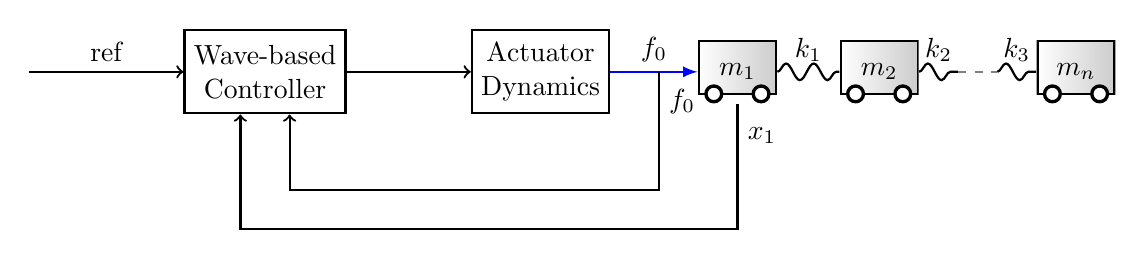
\begin{tikzpicture}[auto]

%Nodes
	\node[pt]	at (0,0)	(ref)													{};
	\node[block] 		(con) 		[right of=ref, node distance=3cm, align=center] 		{Wave-based \\ Controller};
	\node[block] 		(act) 		[right of=con, node distance=3.5cm, align=center]  		{Actuator \\ Dynamics};
	\node[pt]			(for)		[right of=act, node distance=1.5cm]							{};

	
	\node[cart]	(m1)		[right of=for, node distance=1cm]			{$m_1$};
	\node[cart] 	(m2) 		[right of=m1] 	{$m_2$};
	\node[pt] 	(pt1) 		[right of=m2, node distance=1cm] 	{};
	\node[pt] 	(pt2) 		[right of=pt1, node distance=0.5cm] 	{};
	\node[cart] 	(m3) 		[right of=pt2, node distance=1cm] 	{$m_n$};
 	
 	\node[pt]			(int)		[below of=m1, node distance=2cm]							{};
 	\node[pt]			(int2)		[below of=for, node distance=1.5cm]							{};
 	
%Connections	
      \draw[force] (act) -- node {$f_0$} (m1);
 	\draw[line] (ref) -- node {ref}  (con);
 	\draw[line] (con) -- (act);
	\draw[line] (m1) -- node[near start] {$x_1$} (int) -| (con.240);
	\draw[line] (for) -- node[near start] {$f_0$} (int2) -| (con.300);
% 	\draw[line] (minus_x0) -- (k0);
% 	\draw[line] (k0) -- node[] (N2) {$M_{ref}$} (m1);
	
	\draw[spring] (m1) -- node[above] {$k_1$} (m2);
	\draw[spring] (m2) -- node[above] {$k_2$} (pt1);
	\draw[thick,gray, dashed] (pt1) -- (pt2);
	\draw[spring] (pt2) -- node[above] {$k_3$} (m3);
	%\draw[ground] (m1.south west) -- (m3.south east);

\end{tikzpicture}